\documentclass[a4paper,12pt]{report}
% \usepackage[acronym, labelref, glossaries, index, debug]{CEFET}
\usepackage[acronym, labelref]{CEFET}
\addbibresource{Referencias.bib}
\title{Título do Trabalho:}

\subtitle{subtítulo do trabalho (se houver)}

\author{Nome do Autor}  

\date{ANO}

\location{Cidade}

\advisor{Orientador: Título Nome}

\coadvisor{Coorientador: Título Nome (se houver)}

\committeeone{Título Nome\\Instituição}
\committeetwo{Título Nome\\Instituição}
\committeethree{Título Nome\\Instituição}
\committeedate{\today}

\institution{
  Centro Federal de Educação Tecnológica de Minas Gerais
  \\
  Campus Divinópolis
}

\preamble{Trabalho de Conclusão de Curso apresentado no curso de Graduação em Engenharia de Computação do Centro Federal de Educação Tecnológica de Minas Gerais como requisito parcial para obtenção do título de Bacharel em Engenharia de Computação.}
% \newglossaryentry{latex}
{
    name=latex,
    description={Is a markup language specially suited
            for scientific documents}
}

\newglossaryentry{maths}
{
    name=mathematics,
    description={Mathematics is what mathematicians do}
}

%%%%%%%%%%%%%%%%%%%%%%%%%%%%%%%%%%%%%%%%%%%%%%%%%%%%%%
% Se gostou desse template, deixe sua estrela no GitHub:
% https://github.com/lucasmsoares96/Template-Monografia-CEFET-MG
%%%%%%%%%%%%%%%%%%%%%%%%%%%%%%%%%%%%%%%%%%%%%%%%%%%%%%

\usepackage{lipsum}    % gera texto aleatório (remover)

\begin{document}
\maketitle % Capa                    (obrigatório)
% Lombada                            (opcional)

\pretextual
\makecover % folha de rosto               (obrigatório)
\chapter*{Errata}

FERRIGNO, C. R. A. \textbf{Tratamento de neoplasias ósseas apendiculares com
    reimplantação de enxerto ósseo autólogo autoclavado associado ao plasma
    rico em plaquetas}: estudo crítico na cirurgia de preservação de membro em
cães. 2011. 128 f. Tese (Livre-Docência) - Faculdade de Medicina Veterinária e
Zootecnia, Universidade de São Paulo, São Paulo, 2011.

\begin{table}[htb]
    \center
    \footnotesize
    \begin{tabular}{|p{1.4cm}|p{1cm}|p{3cm}|p{3cm}|}
        \hline
        \textbf{Folha} & \textbf{Linha} & \textbf{Onde se lê} & \textbf{Leia-se} \\
        \hline
        1              & 10             & auto-conclavo       & autoconclavo     \\
        \hline
    \end{tabular}
\end{table}%         (opcional)
\makeapproval %                           (obrigatório)
\dedication{Dedico aos meus pais e amigos que me auxiliaram durante o processo de construção deste trabalho.}%    (opcional)
\chapter*{Agradecimentos}
Qual a diferença entre dedicatória e agradecimento? 

A dedicatória na maioria das vezes é um texto curto, sucinto e bem objetivo que destaca a pessoa ou pessoas mais importantes na sua vida. Quando relacionada a vida pessoal, o autor deve agradecer a sua esposa, esposo, filhos, mãe, pai e avós.

No caso dos agradecimentos você não precisa se preocupar com o tamanho do texto. Você pode escrever um pouco mais sobre as pessoas que foram essenciais para seu sucesso. Nos agradecimentos, o autor pode falar da instituição, professores, coordenadores e amigos.

\section*{Exemplo: \href{https://www.abcm.org.br/downloads/TCC_-_Engenharia_Mecanica_2011-1_-_Adriano_Menezes_da_Silva.pdf}{\underline{link}}}

Agradeço primeiramente ao professor Msc. Dilson José Aguiar de Souza pela oportunidade de me orientar na conclusão deste trabalho e me ajudar na realização dos ensaios, além de me auxiliar com muita paciência.

Aos meus pais, Rubem Farias da Silva e Regina Cirinéia Menezes da Silva, por terem me dado força e sustentabilidade financeira no início do curso para chegar a esse momento. Aproveito também a oportunidade para agradecer todo o aporte que me deram em casa e o amor dedicado.

Aos meus irmãos Ana Paula Menezes da Silva e Alexandre Menezes da Silva pelas oportunidades de aprendizagem e troca de experiências.

À minha namorada Nicole Luise Fröehlich Kunsler pela dedicação oferecida, pelos momentos de companheirismo e pela compreensão aos momentos de ausência.

À empresa BLEISTAHL BRASIL METALURGIA S/A, em especial ao funcionário Manfred Kunrath, pela oportunidade de realizar o trabalho de conclusão com materiais fornecidos pela empresa, além de dar aporte financeiro para aquisição de materiais de apoio para a realização dos ensaios.

À empresa LESI Comércio e Representações LTDA, em especial a Fernando Mattes, representante na região da empresa SECO TOOLS que cedeu as ferramentas de corte para os ensaios.

Agradeço à UNISINOS pela cessão dos laboratórios da universidade e ao corpo de funcionários da casa, principalmente aos que me deram apoio e auxílio quando possível e sempre que necessário.% (opcional)
\epigraph{O ontem é história, o amanhã é um mistério, mas o hoje é uma dádiva. É por isso que se chama presente.}{Mestre Oogway}%       (opcional)
\begin{abstract}
    O resumo deve ressaltar o objetivo, o método, os resultados e as conclusões do documento. A ordem e a extensão destes itens dependem do tipo de resumo (informativo ou indicativo) e do tratamento que cada item recebe no documento original. Deve ser precedido da referência do documento, com exceção do resumo inserido no próprio documento, e ser composto de uma sequência de frases concisas, de cunho afirmativo e sem enumeração de tópicos, dado que se recomenda o uso de parágrafo único. As palavras-chave devem figurar logo abaixo do resumo, antecedidas da expressão palavras-chave, e finalizadas também por ponto.
    É importante evitar:
    \begin{enumerate}
        \item símbolos e contrações que não sejam de uso corrente;
        \item fórmulas, equações, diagramas e similares que não sejam absolutamente necessários; quando seu emprego for  imprescindível, deve-se defini-los na primeira vez em que aparecerem.
    \end{enumerate}
    Quanto à extensão, os resumos devem ter:
    \begin{enumerate}
        \item de 150 a 500 palavras os de trabalhos acadêmicos (teses, dissertações e outros) e relatórios técnico-científicos;
        \item de 100 a 250 palavras os de artigos de periódicos;
        \item de 50 a 100 palavras os destinados a indicações breves.
    \end{enumerate}
    Como tratado, o resumo deve ser seguido das palavras representativas do conteúdo do trabalho, isto é, palavras-chave, ou descritores, no idioma em que foi redigido (mínimo 3). Elas devem ser separadas por ponto e virgula e finalizadas com ponto final.
    \\ \\
    \textbf{Palavras-chave:} Palavra-chave 1; Palavra-chave 2; Palavra-chave 3; Palavra-chave 4; Palavra-chave 5.
\end{abstract} %        (obrigatório)
\begin{otherlanguage}{english}
    \begin{abstract}
        Tradução do resumo em português.
        \\ \\
        \textbf{Keywords:} Keywords 1; Keywords 2; Keywords 3; Keywords 4; Keywords 5.
    \end{abstract}
\end{otherlanguage} %      (obrigatório)
\listoffigures %                          (opcional)
\listoftables  %                          (opcional)
\chapter*{Lista de Abreviaturas e Siglas}
\begin{acronym}[xxxxxxxxx]
    \acro{API}{Interface de Programação de Aplicativos, do inglês \textit{Application Programming Interface}}
    \acro{CPU}{Unidade Central de Processamento, do inglês \textit{Central Processing Unit}}
    \acro{DAG}{Grafos Acíclicos Dirigidos, do inglês \textit{Directed Acyclic Graph}}
    \acro{GC}{Coletor de Lixo, do inglês \textit{Garbage Collector}}
    \acro{VM}{Maquina Virtual, do inglês \textit{Virtual Machine}}
\end{acronym}

% Utilização:

% Quando se utiliza o comando \ac{API} pela primeira vez aparece a forma completa do acrônimo, quando se utiliza pela segunda vez aparece apenas a sigla. %        (opcional)
\chapter*{Lista de Símbolos}
\begin{acronym}[xxxxxxxxx]
    \acro{pi}[$\pi$]{Constante matemática que representa a razão entre a circunferência de um círculo e seu diâmetro (3.14159)}
    \acro{alpha}[$\alpha$]{alpha}
    \acro{delta}[$\delta$]{delta}
    \acro{gamma}[$\gamma$]{gamma}
\end{acronym} %      (opcional)
\tableofcontents %                        (obrigatório)

\textual
\chapter{Introdução}

\section{Figuras e Tabelas}
Nos elementos flutuantes, as legendas devem estar alinhadas à esquerda com o comando \textbf{minipage}.

\begin{verbatim}
\begin{table}[!ht]
    \centering
    \begin{minipage}{0.7\textwidth}     <<<<<<<
        \caption{\label{tabela:ComparativoFrameworks}
        Comparação dos Frameworks}
        \resizebox{\textwidth}{!}{
            [...]
        }
        \caption*{\footnotesize Fonte: Elaborado pelo autor, 2023.}
    \end{minipage}
\end{table}
\end{verbatim}

\begin{table}[!ht]
    \centering
    \begin{minipage}{0.7\textwidth}
        \caption{\label{tabela:ComparativoFrameworks}
            Comparação dos Frameworks}
        \resizebox{\textwidth}{!}{
            \begin{tabular}{|l|c|c|c|}
                \hline
                                       & \textbf{MapReduce} & \textbf{Spark} & \textbf{Flink} \\
                \hline
                \textbf{Armazenamento} & Disco              & RAM            & RAM            \\
                \hline
                \textbf{Granularidade} & Grossa             & Grossa         & Fina           \\
                \hline
                \textbf{Estado}        & Sem                & Sem            & Com            \\
                \hline
                \textbf{Processamento} & Lote               & Micro lotes    & Stream         \\
                \hline
                \textbf{Volume}        & Finito             & Finito         & Infinito       \\
                \hline
                \textbf{Linguagem.}    & Java               & Scala          & Java           \\
                \hline
            \end{tabular}
        }
        \caption*{\footnotesize Fonte: Elaborado pelo autor, 2023.}
    \end{minipage}
\end{table}

\section{Citação}

\subsection{Final do texto}
\begin{verbatim}
No atual cenário tecnológico, dados se tornaram um ativo de 
alto valor \cite{gunther2017debating}.
\end{verbatim}

No atual cenário tecnológico, dados se tornaram um ativo de alto valor \cite{gunther2017debating}.

\subsection{Início do texto}
\begin{verbatim}
Segundo \textcite{gunther2017debating} Dados se tornaram um 
ativo de alto valor no atual cenário tecnológico.
\end{verbatim}

Segundo \textcite{gunther2017debating} Dados se tornaram um ativo de alto valor no atual cenário tecnológico.

\section{Alíneas}
Para criar alíneas utilize o comando enumerate, nunca description ou itemize. As alínea devem encerrar com um ponto e vírgula e a última deve encerrar com um ponto final.

\begin{verbatim}
\begin{enumerate}
    \item Primeiro item da alínea;
    \item Segundo item da alínea;
    \item Terceiro item da alínea.
    \begin{enumerate}
        \item Primeiro item da subalínea;
        \item Segundo item da subalínea;
        \item Terceiro item da subalínea.
    \end{enumerate}
\end{enumerate}
\end{verbatim}

\begin{enumerate}
    \item Primeiro item da alínea;
    \item Segundo item da alínea;
    \item Terceiro item da alínea.
          \begin{enumerate}
              \item Primeiro item da subalínea;
              \item Segundo item da subalínea;
              \item Terceiro item da subalínea.
          \end{enumerate}
\end{enumerate}

\section{Customização}

Esse pacote pode ser customizado passando argumentos da seguinte forma:
\begin{verbatim}
\usepackage[acronym, glossaries, index, labelref, debug]{CEFET}
\end{verbatim}

\begin{enumerate}
    \item \textbf{acronym:} adiciona o suporte para lista de abreviaturas e siglas;
    \item \textbf{glossaries:} adiciona o suporte para glossário;
    \item \textbf{index:} adiciona o suporte para índice de assunto;
    \item \textbf{labelref:} \verb|\ref{fig:1}| retorna Figura 1 em vez de 1 para todas as referências;
    \item \textbf{debug:} Ativa as réguas e os quadros para melhorar a visualização das medidas.
\end{enumerate}

\section{Namedref}
\begin{verbatim}
Exemplo de utilização do \textbf{namedref} para a 
\ref{tabela:ComparativoFrameworks}.
\end{verbatim}
Exemplo de utilização do \textbf{namedref} para a \ref{tabela:ComparativoFrameworks}.
\chapter{Referencial Teórico}
\lipsum[1] \ref{fig:Stack} \cite{anuradha2015brief}

\begin{figure}[!htb]
    \centering
    \begin{minipage}{0.8\textwidth}
        \caption{\label{fig:Stack} Pilha de Tecnologias utilizadas em Big Data}
        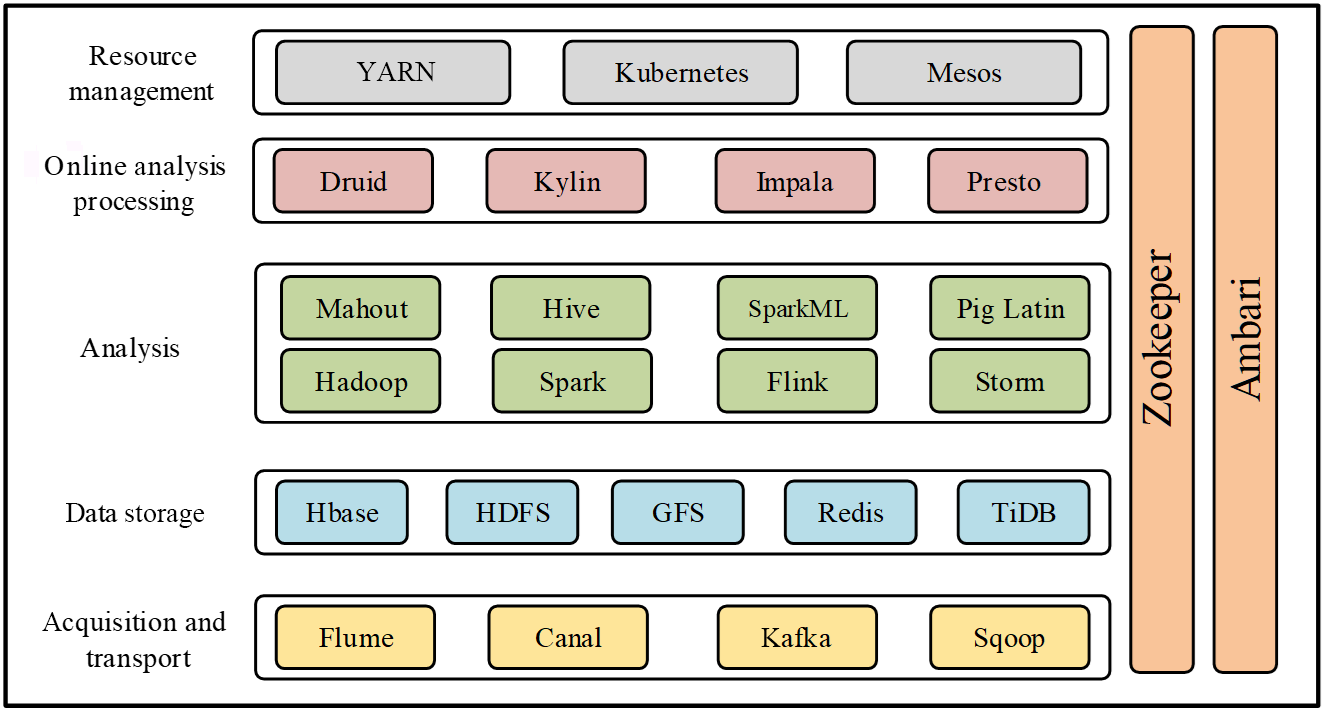
\includegraphics[width=\textwidth]{Imagens/Stack.png}
        \caption*{\footnotesize Fonte: \textcite{sun2023survey}.}
    \end{minipage}
\end{figure}

\lipsum[6]

\section{Seção}
\lipsum[2]
\cite{anuradha2015brief}
\subsection{SubSeção}
\lipsum[3]
\cite{anuradha2015brief}
\subsubsection{SubSubSeção}
\lipsum[4]
\cite{zaharia2012resilient}
% \chapter{Metodologia}

\section{Introduction}
In this example, several keywords\index{keywords} will be used which
are important and deserve to appear in the Index\index{Index}. Terms like generate\index{generate} and some\index{others} will also
show up. Terms in the index can also be nested \index{Index!nested}

\section{Second section}
This second section\index{section} may include some special word,
and expand the ones already used\index{keywords!used}.
% \chapter{Resultados}
The \gls{latex} typesetting markup language is specially suitable
for documents that include \gls{maths}.
% \input{2-Textual/5-Conclusao.tex}

\postextual
\clearpage\pagestyle{empty}
\printbibliography %                 (obrigatório)
% \printglossaries %                   (opcional)
\clearpage\pagestyle{plain}
\chapter*{Apêndice A -- Nome}
Material criado pelo autor % (opcional)
\chapter*{Anexo A -- Nome}
Material \textbf{não} criado pelo autor. %    (opcional)
% \printindex %                        (opcional)

\end{document}